\part{Limits and Continuity}

\chapter{Basic Limits}

\section{Basic Limits}

Suppose we have a function $ y = f(x) $. The limit of $ f(x) $ as $ x $ approaches the number $ a $, denoted $ \lim\limits_{x \rightarrow a}f(x) $. \\

For example, suppose we wanted to determine $ \lim\limits_{x \rightarrow 3}x^2 $. \\

\begin{table}[H]
	\centering
	\begin{tabular}{|c|c|} \hline
		\textbf{$ x $ approaches 3 from the left} & \textbf{$ x $ approaches 3 from the right} \\ \hline
		$ f(2.9) = 8.41 $                         & $ f(3.1) = 9.61 $                          \\ \hline
		$ f(2.99) = 8.9401 $                      & $ f(3.01) = 9.0601 $                       \\ \hline
		$ f(2.999) = 8.994001 $                   & $ f(3.001) = 9.006001 $                    \\ \hline
	\end{tabular}
\end{table}

No matter which way we approach from, as $ x $ gets close 3, we can see that $ x^2 $ gets very close to 9. \\

\begin{exercise}\nonumber
	Find  $ \lim\limits_{x \rightarrow 0}f(x) $ where \\
	\begin{align}
		f(x) = \begin{cases}
			cos(x) & x \ne 0 \\
			-1     & x = 0
		\end{cases}
	\end{align}

	\begin{figure}[H]
		\centering
		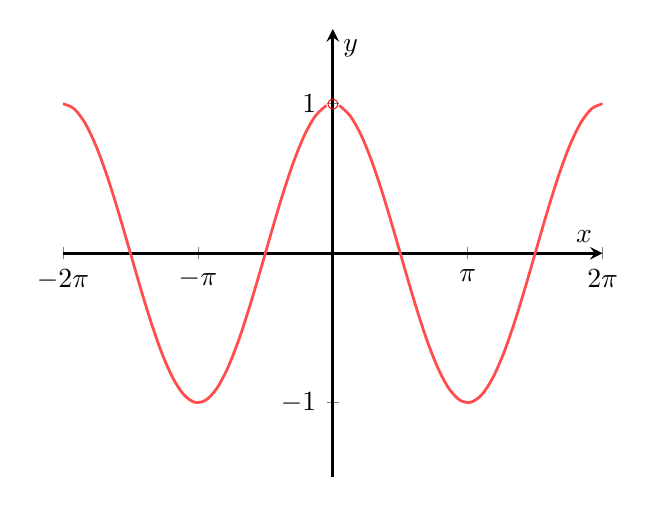
\begin{tikzpicture}
			\begin{axis}[
					xlabel={$ x $}, ylabel={$ y $},
					xmin=-2*pi, xmax=2*pi,
					ymin=-1.5, ymax=1.5,
					xtick={-6.28319, -3.14159, 0, 3.14159, 6.28319},
					xticklabels={$-2\pi$, $-\pi$, $0$, $\pi$, $2\pi$},
					line width=1pt,
					axis lines=center,
				]
				\addplot[smooth,domain=-2*pi:-0.15, red!70]{cos(deg(x))};
				\addplot[smooth,domain=0.15:2*pi, red!70]{cos(deg(x))};
			\end{axis}
			\node at (3.43,4.72) [red,circle,inner sep=1pt]{$\circ$};
		\end{tikzpicture}
	\end{figure}

	\begin{gather*}
		\lim\limits_{x \rightarrow 0}f(x) = 1 \\
		f(0) = -1
	\end{gather*}
\end{exercise}

\section{Law of Limits}

\begin{theorem}[Law of Limits]
	\begin{align}
		 & \lim\limits_{x \rightarrow a}(f+g)(x) = \lim\limits_{x \rightarrow a}f(x) + \lim\limits_{x \rightarrow a}g(x)                          \\
		 & \lim\limits_{x \rightarrow a}(f-g)(x) = \lim\limits_{x \rightarrow a}f(x) - \lim\limits_{x \rightarrow a}g(x)                          \\
		 & \lim\limits_{x \rightarrow a}(fg)(x) = \lim\limits_{x \rightarrow a}f(x) \cdot \lim\limits_{x \rightarrow a}g(x)                       \\
		 & \lim\limits_{x \rightarrow a}\left({f \over g}\right)(x) = {\lim\limits_{x \rightarrow a}f(x) \over \lim\limits_{x \rightarrow a}g(x)}
	\end{align}
\end{theorem}

\begin{exercise}\nonumber
	Evaluate $ \lim\limits_{x \rightarrow 0}xsin\left({1 \over x}\right) $. \\
	\begin{gather*}
		-1 \le  sin\left({1 \over x}\right) \le 1 \\
		-x \le xsin\left({1 \over x}\right) \le x \\
		\lim\limits_{x \rightarrow 0}-x \le \lim\limits_{x \rightarrow 0}xsin\left({1 \over x}\right) \le \lim\limits_{x \rightarrow 0}x \\
		\therefore \lim\limits_{x \rightarrow 0}xsin\left({1 \over x}\right) = 0
	\end{gather*}
\end{exercise}

\section{One-sided Limits}

$ x $ can approach the value a in two ways: \\

\begin{itemize}
	\item
	      left-hand limit: $ \lim\limits_{x \rightarrow a^-}f(x) $ \\

	\item
	      right-hand limit: $ \lim\limits_{x \rightarrow a^+}f(x) $ \\
\end{itemize}

We can tighten our definition of the limit of a function $ f(x) $ as $ x $ approaches $ a $. If the left-hand and right-hand limits of $ f(x) $ are both equal to a number $ L $, then we say that $ \lim\limits_{x \rightarrow a}f(x) $ exists and is equal to $ L $. \\

\begin{exercise}\nonumber
	Consider the piecewise function given by \\
	\begin{align}
		f(x) = \begin{cases}
			x          & x < 1 \\
			-1         & x = 1 \\
			\sqrt{x-1} & x > 1
		\end{cases}
	\end{align}

	(a) $ \lim\limits_{x \rightarrow 1^-}f(x) = 1 $ \\

	(b) $ \lim\limits_{x \rightarrow 1^+}f(x) = 0 $ \\

	(c) $ f(1) = -1 $ \\

	(d) Does $ \lim\limits_{x \rightarrow 1}f(x) $ exist? No.
\end{exercise}

\chapter{Continuity}

\section{Continuity}

It seems like sometimes we can evaluate a limit by just plugging in, but sometimes we can't! \\

\begin{exercise}\nonumber
	Evaluate $ \lim\limits_{x \rightarrow 1}\left(ln(\sqrt{x}) + {1 \over x}\right) $. \\
	\begin{align}
		 & \lim\limits_{x \rightarrow 1}\left(ln(\sqrt{x}) + {1 \over x}\right) \\
		 & = ln\left(\sqrt{x} + {1 \over x}\right)                              \\
		 & = ln\left(\sqrt{1}\right) + {1 \over 1}                              \\
		 & = 0 + 1                                                              \\
		 & = 1
	\end{align}
\end{exercise}

A function is continuous at a point a if each of the following conditions hold: \\

\begin{enumerate}
	\item
	      $ \lim\limits_{x \rightarrow a}f(x) $ exists \\

	\item
	      $ f(a) $ exists \\

	\item
	      $ \lim\limits_{x \rightarrow a}f(x) = f(a) $ \\
\end{enumerate}

\section{Discontinuity}

Kinds of discontinuities: \\

\begin{figure}[H]
	\centering
	\begin{tikzpicture}[scale=0.7]
		\draw[->] (-5,0) -- (4,0) node[right] {$ x $};
		\draw[->] (0,-4) -- (0,4) node[above] {$ y $};
		\draw[very thick,color=red,domain=-4.5:-1.3] plot (\x,{1 / (\x + 1)});
		\draw[very thick,color=red,domain=-0.7:3] plot (\x,{1 / (\x + 1)});
		\draw[very thick,densely dashed,color=red] (-1,4)--(-1,-4);
	\end{tikzpicture}
	\caption{essential}
\end{figure}

\begin{figure}[H]
	\centering
	\begin{tikzpicture}
		\begin{axis}[
				xlabel={$ x $}, ylabel={$ y $},
				xmin=-2*pi, xmax=2*pi,
				ymin=-1.5, ymax=1.5,
				xtick={-6.28319, -3.14159, 0, 3.14159, 6.28319},
				xticklabels={$-2\pi$, $-\pi$, $0$, $\pi$, $2\pi$},
				line width=1pt,
				axis lines=center,
			]
			\addplot[smooth,domain=-2*pi:1.07, red!70]{sin(deg(x))};
			\addplot[smooth,domain=1.2:2*pi, red!70]{sin(deg(x))};
			\node at (742,240) [red,circle,inner sep=1pt]{$\circ$};
		\end{axis}
	\end{tikzpicture}
	\caption{removable}
\end{figure}

\begin{figure}[H]
	\centering
	\begin{tikzpicture}[scale=0.5,yscale=0.3]
		\draw[->] (-10,0) -- (6,0) node[right] {$ x $};
		\draw[->] (0,-5) -- (0,20) node[above] {$ y $};
		\draw[very thick,color=red,domain=-9:-2.1] plot (\x,{0.5 * \x + 3});
		\draw[very thick,color=red,domain=-2:2] plot (\x,{0});
		\draw[very thick,color=red,domain=2.1:4] plot (\x,{\x^2 - 1});
		\foreach \point in {(-2,0),(2,0)} {
				\node at \point [red,circle,fill,inner sep=1.5pt]{};
			}
		\foreach \point in {(-2,2),(2,3)} {
				\node at \point [red,circle,inner sep=1.5pt]{$\circ$};
			}
	\end{tikzpicture}
	\caption{jump}
\end{figure}

So far, we know that evaluating $ \lim\limits_{x \rightarrow a}f(x) $ is easy if $ f(x) $ is continuous at $ a $. But what if it isn't? The limit may still exist. \\

\begin{exercise}\nonumber
	Evaluate the following limits. \\

	(a) $ \lim\limits_{x \rightarrow 3^+}{1 \over 3-x} = -\infty $ \\

	(b) $ \lim\limits_{x \rightarrow 3^-}{1 \over 3-x} = \infty $ \\

	(c) $ \lim\limits_{x \rightarrow 0^+}ln(x) = -\infty $ \\

	(d) $ \lim\limits_{x \rightarrow -{\pi \over 2}^+}sec(x) = \infty $
\end{exercise}

A function doesn't have to go to $ \pm \infty $ at a discontinuity though. Consider, for instance, evaluating $ \lim\limits_{x \rightarrow 3}{x^2-x-6 \over x-3} $. Plugging in $ x = 3 $ gives us "$ 0 / 0 $", which is known as an indeterminate form. \\

A good first step is to factor where possible. Once we cancel the factor $ x - 3 $ on top and bottom, this function is just the function $ f(x) = x + 2 $, but with a hole at $ x = 3 $. The hole is there because we cannot ignore that the original form of the function had issues at $ x = 3 $. \\

\begin{exercise}\nonumber
	Evaluate the following limits. \\

	(a)
	\begin{align}
		 & \lim\limits_{x \rightarrow 3}{x^2-x-6 \over x-3}      \\
		 & = \lim\limits_{x \rightarrow 3}{(x-3)(x+2) \over x-3} \\
		 & = \lim\limits_{x \rightarrow 3}{x+2}                  \\
		 & = 5
	\end{align}

	\begin{figure}[H]
		\centering
		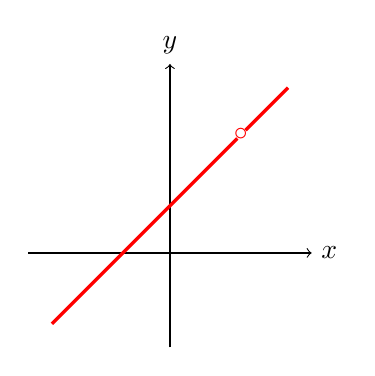
\begin{tikzpicture}[scale=0.3]
			\draw[->] (-6,0) -- (6,0) node[right] {$ x $};
			\draw[->] (0,-4) -- (0,8) node[above] {$ y $};
			\draw[very thick,color=red,domain=-5:2.85] plot (\x,{\x + 2});
			\draw[very thick,color=red,domain=3.2:5] plot (\x,{\x + 2});
			\node at (3,5) [red,circle,inner sep=1.5pt]{$\circ$};
		\end{tikzpicture}
	\end{figure}

	(b)
	\begin{align}
		 & \lim\limits_{x \rightarrow -1}{x^3 - 11x^2 + 8x + 20 \over x + 1} \\
		 & = \lim\limits_{x \rightarrow -1}{(x+1)(x^2-12x+20) \over x + 1}   \\
		 & = (-1)^2 - 12(-1) + 20                                            \\
		 & = 33
	\end{align}
	\\

	(c)
	\begin{align}
		 & \lim\limits_{x \rightarrow 4}{\sqrt{x+5} - 3 \over x-4}                                              \\
		 & = \lim\limits_{x \rightarrow 4}{({{\sqrt{x+5}-3} \over {x-4}})({{\sqrt{x+5}+3} \over \sqrt{x+5}+3})} \\
		 & = \lim\limits_{x \rightarrow 4}{x-4 \over (x-4)(\sqrt{x+5}+3)}                                       \\
		 & = {1 \over \sqrt{9} + 3}                                                                             \\
		 & = {1 \over 6}
	\end{align}
	\\

	(d)
	\begin{align}
		 & \lim\limits_{x \rightarrow 2}{{1 \over x-4} + {1 \over 2} \over x-2}                     \\
		 & = \lim\limits_{x \rightarrow 2}{{{2+(x-4)} \over {2(x-4)}} \over x-2}                    \\
		 & = \lim\limits_{x \rightarrow 2}{\left({x-2 \over 2x-4}\right)\left({1 \over x-2}\right)} \\
		 & = \lim\limits_{x \rightarrow 2}{1 \over 2(x-4)}                                          \\
		 & = {1 \over 2(-2)}                                                                        \\
		 & = -{1 \over 4}
	\end{align}
\end{exercise}

\chapter{The Fundamental Sine Limit}

\section{The Fundamental Sine Limit}

Consider the following limit:

$$
	\lim\limits_{x \rightarrow 0}{sin(x) \over x}
$$

We can quickly see that this is a "$ 0 / 0 $" limit, and therefore is indeterminate. We can't factor anything or otherwise simplify the expression to get rid of the issue. \\

\begin{figure}[H]
	\centering
	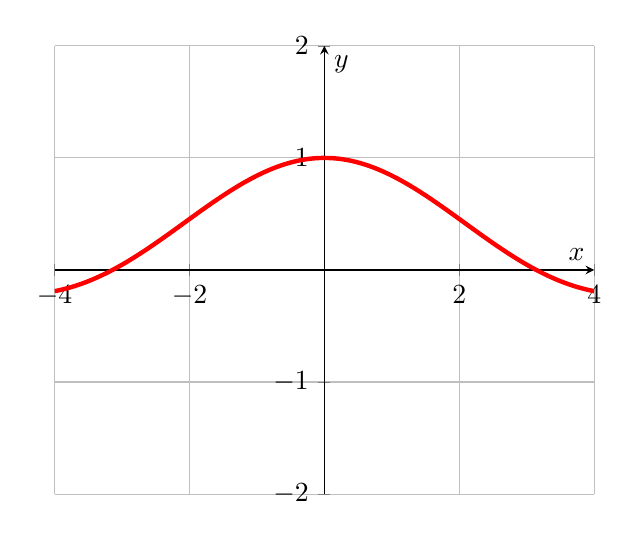
\begin{tikzpicture}[scale=1]
		\begin{axis}[
				grid=both,
				xmin=-4,
				xmax=4,
				ymin=-2,
				ymax=2,
				xlabel=$x$,
				ylabel=$y$,
				axis lines=center,
				>=stealth
			]
			\addplot[
				domain=-4:4,
				red,
				ultra thick,
				samples=100,
			] plot[smooth] {sin(deg(x))/x};
		\end{axis}
	\end{tikzpicture}
	\caption{$ sin(x) \over x $}
\end{figure}

It is pretty clear from the graph that \\

\begin{theorem}[The Fundamental Sine Limit]
	\begin{align}
		\lim\limits_{x \rightarrow 0}{sin(x) \over x} = \lim\limits_{x \rightarrow 0}{x \over sin(x)} = 1
	\end{align}
\end{theorem}

\begin{exercise}\nonumber
	Evaluate the following limits. \\

	(a)
	\begin{align}
		 & \lim\limits_{t \rightarrow 0}{5sin(t) \over 2t}                     \\
		 & = \lim\limits_{t \rightarrow 0}{{5 \over 2} \cdot {sin(t) \over t}} \\
		 & = {5 \over 2}
	\end{align}
	\\

	(b)
	\begin{align}
		 & \lim\limits_{\theta \rightarrow 0}{\theta \over sin(4\theta)}                 \\
		 & = \lim\limits_{\theta \rightarrow 0}{4\theta \over 4sin(4\theta)}             \\
		 & = \lim\limits_{\theta \rightarrow 0}{{1 \over 4}{4\theta \over sin(4\theta)}} \\
		 & = {1 \over 4}
	\end{align}
	\\

	(c)
	\begin{align}
		 & \lim\limits_{x \rightarrow -1}{sin^2(x+1) \over (x+1)^2}                          \\
		 & = \lim\limits_{x \rightarrow -1}{{sin(x+1) \over x+1} \cdot {sin(x+1) \over x+1}} \\
		 & = 1
	\end{align}
	\\

	(d)
	\begin{align}
		 & \lim\limits_{x \rightarrow 0}{sin(3x) \over sin(2x)}                                          \\
		 & = \lim\limits_{x \rightarrow 0}{{sin(3x) \over 3} \cdot {2x \over sin(2x)} \cdot {3 \over 2}} \\
		 & = {3 \over 2}
	\end{align}
	\\

	(e)
	\begin{align}
		 & \lim\limits_{\theta \rightarrow 0}{100\theta \over tan(3\theta)}                                                 \\
		 & = \lim\limits_{\theta \rightarrow 0}{10\theta \cdot {cos(3\theta) \over sin(3\theta)}}                           \\
		 & = \lim\limits_{\theta \rightarrow 0}{{3\theta \over sin(3\theta)} \cdot {1 \over 3} \cdot 10 \cdot cos(3\theta)} \\
		 & = 1 \cdot {10 \over 3} \cdot 1                                                                                   \\
		 & = {10 \over 3}
	\end{align}
	\\

	(f)
	\begin{align}
		 & \lim\limits_{h \rightarrow 0}{cos(h)-1 \over h}                                                        \\
		 & = \lim\limits_{h \rightarrow 0}{\left({cos(h)-1 \over h}\right)\left({cos(h)+1 \over cos(h)+1}\right)} \\
		 & = \lim\limits_{h \rightarrow 0}{cos^2h - 1 \over h(cos(h) + 1)}                                        \\
		 & = \lim\limits_{h \rightarrow 0}{-sin^2h \over h\left(cos(h) + 1\right)}                                \\
		 & = \lim\limits_{h \rightarrow 0}{-{sin(h) \over h} \cdot {sin(h) \over cos(h) + 1}}                     \\
		 & = -1 \cdot {0 \over 1+1}                                                                               \\
		 & = 0
	\end{align}
\end{exercise}

\chapter{Limits Approaching $ \pm \infty $}

\section{Limits Approaching $ \pm \infty $}

Sometimes, we will be interested in determining what happens as $ x $ gets really big, either in the positive or negative direction. \\

\begin{exercise}\nonumber
	Evaluate the following limits. \\

	(a) $ \lim\limits_{x \rightarrow \infty}{1 \over x} = 0 $ \\

	(b) $ \lim\limits_{x \rightarrow -\infty}{1 \over x} = 0 $ \\

	(c) $ \lim\limits_{x \rightarrow -\infty}{401 \over x^{203}} = 0 $ \\

	(d) $ \lim\limits_{x \rightarrow -\infty}{-238 \over 23x^{1/4}} = 0 $
\end{exercise}

For problems like $ \lim\limits_{x \rightarrow \infty}{2x^2 + 3x + 1 \over x^2 - 10x + 100} $, a good first step is to divide the top and the bottom by the highest power of $ x $ appearing in the denominator. \\

\begin{exercise}\nonumber
	Evaluate the following limits. \\

	(a)
	\begin{align}
		 & \lim\limits_{x \rightarrow \infty}{2x^2 + 3x + 1 \over x^2 - 10x + 100}                                            \\
		 & = \lim\limits_{x \rightarrow \infty}{\left({2x^2+3x+1 \over x^2-10x+100}\right)\left({1/x^2 \over 1/x^2}\right)}   \\
		 & = \lim\limits_{x \rightarrow \infty}{\left({2x^2+3x+1 \over x^2-10x+100}\right)\left({1/x^2 \over 1/x^2}\right)}   \\
		 & = \lim\limits_{x \rightarrow \infty}{{2 + {3 \over x} + {1 \over x^2}} \over {1 - {10 \over x} + {100 \over x^2}}} \\
		 & = {2 \over 1}                                                                                                      \\
		 & = 2
	\end{align}
	\\

	(b)
	\begin{align}
		 & \lim\limits_{x \rightarrow -\infty}{3 - 2x^3 \over 1 + x + x^2}                                            \\
		 & = \lim\limits_{x \rightarrow -\infty}{\left({3-2x^3 \over 1+x+x^2}\right)\left({1/x^2 \over 1/x^2}\right)} \\
		 & = \lim\limits_{x \rightarrow -\infty}{{3 \over x^2} - 2x \over {{1 \over x^2} + {1 \over x} + 1}}          \\
		 & = \lim\limits_{x \rightarrow -\infty}{-2x \over 1}                                                         \\
		 & = \infty
	\end{align}
	\\

	(c)
	\begin{align}
		 & \lim\limits_{x \rightarrow \infty}{\sqrt{x^2 - x + 1}}                                                                    \\
		 & = \lim\limits_{x \rightarrow \infty}{\left(\sqrt{x^2-x+1}-x\right)\left({\sqrt{x^2-x+1}+x \over \sqrt{x^2-x+1}+x}\right)} \\
		 & = \lim\limits_{x \rightarrow \infty}{(x^2-x+1)-x^2 \over \sqrt{x^2-x+1}+x}                                                \\
		 & = \lim\limits_{x \rightarrow \infty}{x+1 \over \sqrt{x^2-x+1}+x}                                                          \\
		 & = \lim\limits_{x \rightarrow \infty}{\left({x+1 \over \sqrt{x^2-x+1}+x}\right)\left({1/x \over 1/x}\right)}               \\
		 & = \lim\limits_{x \rightarrow \infty}{-1 + {1 \over x} \over {\sqrt{x^2-x+1} \over x} + 1}                                 \\
		 & = \lim\limits_{x \rightarrow \infty}{-1 + {1 \over x} \over \sqrt{{x^2-x+1} \over x^2} + 1}                               \\
		 & = \lim\limits_{x \rightarrow \infty}{-1 \over \sqrt{1} + 1}                                                               \\
		 & = -{1 \over 2}
	\end{align}
	\\

	(d)
	\begin{align}
		 & \lim\limits_{t \rightarrow \infty}{\sqrt{3t^2 + 2t + 5} + t} \\
		 & = \infty
	\end{align}
\end{exercise}